\section{Context}


\begin{frame}
\frametitle{Secure Component and Embedded Cryptography}
\textbf{A piece of hardware with security properties.}\\
\textbf{It usually embeds cryptography to provide security services (authentication, signature, secure messaging with terminals...)}
\begin{columns}
\begin{column}{0.5\textwidth}
\uncover<2->{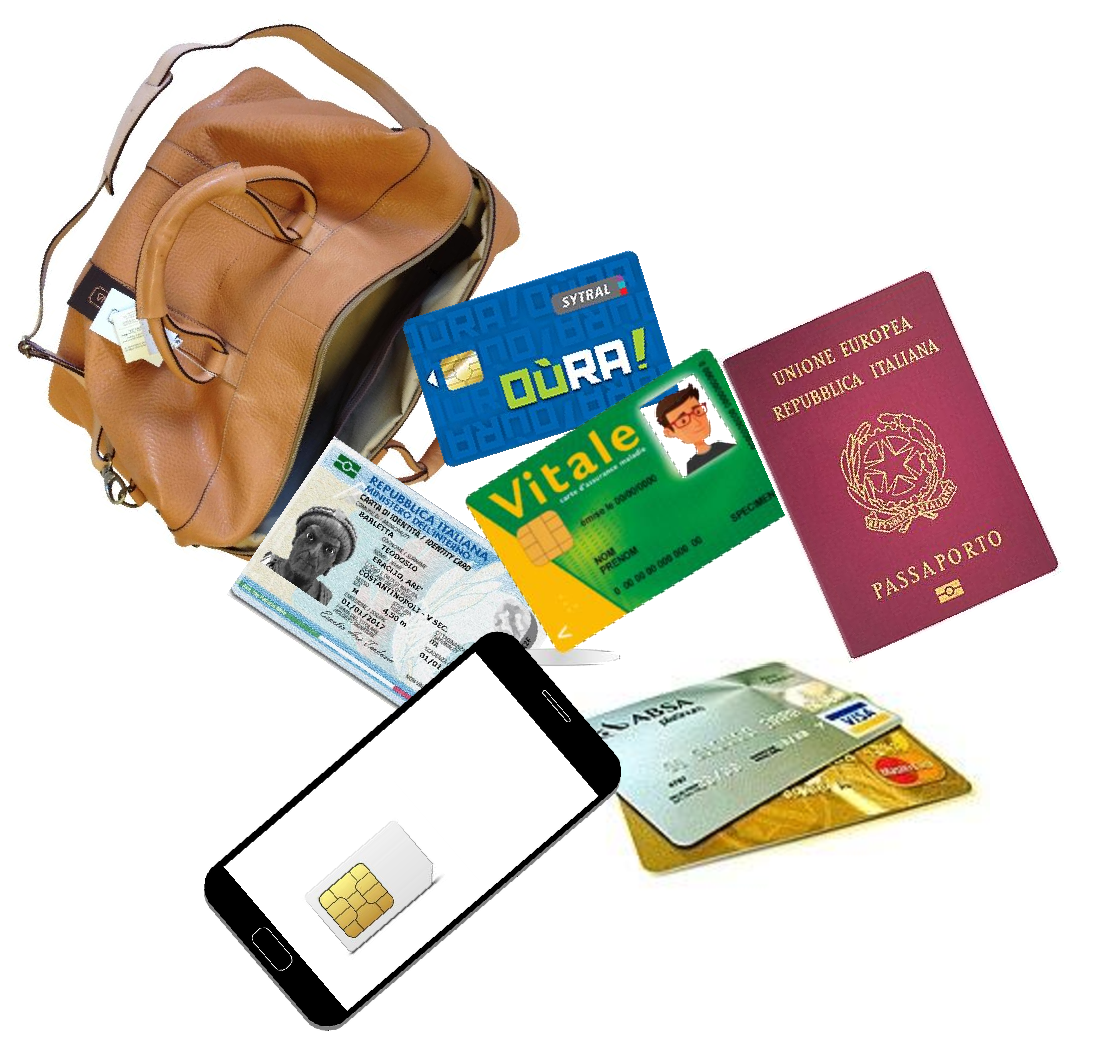
\includegraphics[width = \textwidth]{figures/smartcards.pdf}}
\end{column}
\begin{column}{0.5\textwidth}
\begin{itemize}
\item Sensitive applications: ID cards, credit cards, transport cards, health cards, SIM
\item Pervasive aspect: several billion smartcards sold par year
\item Hard to update
\item Hostile environment
\end{itemize}
\end{column}
\end{columns}
\uncover<3->{$\Rightarrow$ Requires protection against very high-level attacker}
\end{frame}

\begin{frame}
\frametitle{Security Certification}
\centering
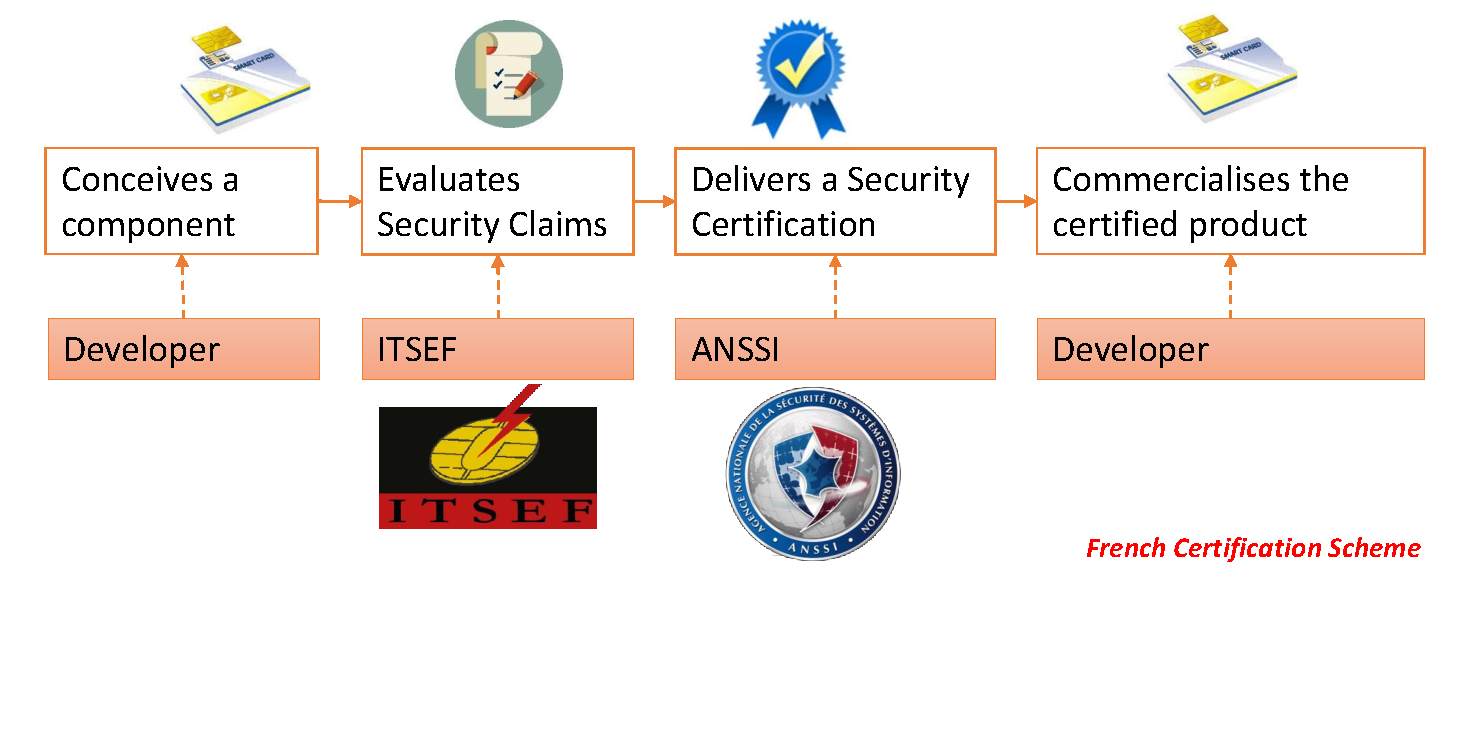
\includegraphics[width = .9\textwidth]{figures/ITSEF_nobody.pdf}
\begin{itemize}
\item Standardized Evaluation (\eg ISO/IEC 15408 - Common Criteria)
\item Assigns an Evaluation Assurance Level (EAL)
\item The evaluator checks the Security Assurance Requirements (SAR), \eg ADV, ALC, AVA, ...
\item AVA: vulnerability assessment (penetration testing $\rightarrow$ attack potential rating)
\end{itemize}
\end{frame}

\begin{frame}
\frametitle{Side-Channel Vulnerability of Embedded Cryptography}
\centering
\scalebox{0.6}{
\begin{tikzpicture}[ ->, node distance = 3cm,
					decoration = {snake,   % <-- added
                    pre length=3pt,post length=7pt,% <-- for better looking of arrow,
                    }]
\node [data] (plaintext){plaintext};
\node [cipher, right of=plaintext] (AES) {\only<1>{AES}\only<2->{
\includegraphics[width = \textwidth]{figures/Computer_Chip-512.png}\\Intermediate Computations}};
\node [data, right of=AES] (ciphertext){ciphertext};
\node [ above right of=AES] (Conso) {Power Consumption};
\node [ below right of=AES] (EM) {Electromagnetic Irradiation};
\node [ above left of=AES] (Time) {Time Duration};
\node [ below left of=AES] (Sound) {Sound Emanation};
\path[draw=blue, very thick, decorate] (AES) -> (Sound);
\path[draw=blue, very thick, decorate] (AES) -> (Time);
\path[draw=blue, very thick, decorate] (AES) -> (Conso);
\path[draw=blue, very thick, decorate] (AES) -> (EM);
\draw [arrow] (plaintext) -- (AES);
\draw [arrow] (AES) -- (ciphertext);
\end{tikzpicture}
}

\begin{columns}
\begin{column}{.5\textwidth}
\textbf{Classical Cryptanalysis}
\begin{itemize}
\item Black box (input, output)
\item Formal attacker model (oracle, knowledge, ...)
\item Computational complexity to perform the attack (\eg $2^{126.1}$ operations to break AES-128 \cite{bogdanov})
\end{itemize}
\end{column}
\begin{column}{.5\textwidth}
\textbf{Side-Channel Cryptanalysis}
\begin{itemize}
\item White box (input, output, side-channel observations of intermediate computations)
\item Attacker with a certain equipment, expertise, knowledge of the embedded device, available time...
\item In Common Criteria: the cotation table of the attack
\end{itemize}
\end{column}
\end{columns}

% con i 5 punti della tesi per definire un attacco
\end{frame}

\begin{frame}
\frametitle{Side-Channel Attacks}
\begin{itemize}
\item \textbf{the physical nature of the exploited signals}: \only<1>{power consumption, electromagnetic irradiation}\only<2>{\textcolor{red}{power consumption, electromagnetic irradiation}}, time, sound, temperature, \dots
\item \textbf{the chosen sensitive variable/s} $Z$:
\begin{itemize}
\item $Z = K$ a secret key chunk
\item \only<1>{$Z = f(K,E)$}\only<2>{\textcolor{red}{$Z = f(K,E)$}} a variable depending on a secret key chunk and on a piece of public information
\item an operation (\eg $Z \in \{ square, multiply, \dots\}$)
\item a register 
\item \only<1>{$Z^\prime = \varphi(Z)$}\only<2>{\textcolor{red}{$Z^\prime = \varphi(Z)$}} a non-injective function of any sensitive variable (\eg $f = \mathrm{HW}$ Hamming Weight)
\end{itemize}
\item \textbf{the strategy family}: simple attacks, collision attacks, \only<1>{differential/advanced attacks}\only<2>{\textcolor{red}{differential/advanced attacks}}
\item \textbf{the shape of the attack}: horizontal attacks, vertical attacks
\item \textbf{the attacker knowledge}: \only<1>{profiling}\only<2>{\textcolor{red}{profiling}}, non-profiling attacks
\end{itemize}
\end{frame}





%\begin{frame}
%\vspace{-15pt}
%\frametitle{Context}
%\begin{block}{Side-Channel Attacks (SCAs)}
%\begin{itemize}
%\item Target: a physical implementations of cryptographic primitives 
%\item Means: observable physical variations (timing information, power consumption, electromagnetic irradiation, etc.)
%\item Goal: retrieve secret data (ex: cryptographic key)
%\end{itemize}
%\end{block}
%
%\begin{block}{Notations}
%\begin{itemize}
%\item Side-channel traces: realizations of a random variable $\XXX \in \mathbb{R}^D$  (column vector)
%\item Target: a \emph{sensitive} variable $Z = f(P,K)\in\sensVarSet$ 
%\end{itemize}
%\end{block}
%\vspace{-5pt}
%\begin{block}{Profiling attack scenario}
%Exploits labelled traces $(\sss[z_i]{i})_{i=1}^N$ to characterize the signals in function of $z_i$.\\
%\emph{"a trace $\sss[z]{}$ belongs to the class $z$"}
%\end{block}
%%\begin{small}
%%\emph{Example: Gaussian Template Attack} 
%%\begin{itemize}
%%\item Profiling phase: estimate the parameters $\{(\mumumu_z,\Sigma_z)\}_{z\in\sensVarSet}$ of multivariate Gaussian distributions
%%\item Attack phase: rank key hypothesis through maximum likelihood
%%\end{itemize}
%%\end{small}
%
%
%
%\end{frame}
%
%
%
%
%%\begin{frame}
%%\vspace{-5pt}
%%\frametitle{Points of Interest}
%%\vspace{-10pt}
%%
%%\begin{block}{Problem}
%%Highly multi-dimensional side-channel traces (algorithm, instruments sampling rate, etc.)\\
%%$\longrightarrow$ affects attack complexity
%%\end{block}
%%
%%\includegraphics[width = 0.4\textwidth]{figures/power_trace.pdf}
%%\only<2>{
%%\includegraphics[width = 0.4\textwidth]{figures/SNR_trace.pdf}
%%}
%%
%%\begin{block}{Which part characterize?}
%%Only (relatively) few points depend on the target: the \emph{Points of Interest (PoIs)}
%%\end{block}
%%
%%\pause
%%\begin{block}{How to find them?}
%%A first answer: statistical tests.\\
%%For example estimating the SNR:
%%\begin{equation}
%%\SNR = \frac{\var(\esper[\XXX\vline Z])}{\esper[\var(\XXX\vline Z)]}
%%\end{equation}
%%\end{block}
%%
%%
%%\end{frame}
%
%
%
%
%\begin{frame}
%\frametitle{Dimensionality Reduction}
%
%\begin{block}{Problem}
%Highly multi-dimensional side-channel traces (algorithm, sampling rate, etc.)\\
%$\longrightarrow$ affect attack complexity
%\end{block}
%
%\begin{block}{Goal}
%Perform a preprocessing via an opportune \emph{extractor} $\extract:\mathbb{R}^D\rightarrow \mathbb{R}^C$ in order to:
%\begin{itemize}
%\item Reduce memory and time complexity (ameliorate the attacks efficiency in terms of required samples)
%\item Enhance contribution of the Points of Interest (PoI, those that depend on the target) to concentrate information over few points (ameliorate the attacks efficiency in terms of required traces)
%\end{itemize}
%\end{block}
%
%%\begin{block}{Extractor}
%%\begin{equation}
%%\extract:\mathbb{R}^D\rightarrow \mathbb{R}^C
%%\end{equation}
%%\end{block}
%
%
%\end{frame}
%
%\begin{frame}
%\frametitle{Literature}
%Two typologies of extractors in literature
%\begin{block}{Selecting Extractors}
%$\extract$ performs a sub-sampling
%\begin{itemize}
%\item Sum of Differences (SOD) \cite{Chari2003}
%\item Signal-to-Noise Ratio (SNR) \cite{mangard2008power}
%\item Sum of Squared $t$-differences (SOST), $t$-test, $F$-test,... \cite{gierlichs2006templates,bar2010improved,choudary2014efficient}
%\end{itemize}
%\end{block}
%
%\begin{block}{Projecting Extractors}
%$\extract(\sss[]{}) = A\sss[]{} \mbox{ with } A \in M_{\mathbb{R}}(\newTraceLength, \traceLength)$
%\begin{itemize}
%\item Principal Component Analysis (PCA) \cite{TAprincipal,Batina2012}
%\item Linear Discriminant Analysis (LDA) \cite{Standaert2008,lessIsMore}
%\end{itemize}
%\end{block}
%
%\end{frame}

